\documentclass{standalone}
\usepackage{../preamble}

\begin{document}
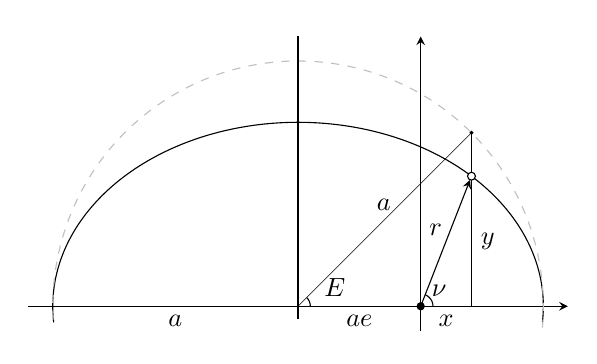
\begin{tikzpicture}[every node/.style={scale=0.95}]
  \begin{axis}[
      xmin=-3.2,xmax=1.2,ymin=-0.2,ymax=2.2,
      axis lines=middle,
      ytick = {0},
      xtick = {0},
      axis equal image,
      clip=false,
      % ylabel={$y$},
      % xlabel={$x$},
    ]
    \def\a{2}
    \def\b{1.5}
    \def\c{1}
    \def\angle{45}
    \def\ymax{\pgfkeysvalueof{/pgfplots/ymax}}
    \def\ymin{\pgfkeysvalueof{/pgfplots/ymin}}
    \addplot[thin,samples=400,domain=-5:185] ({\a*cos(x)-\c},{\b*sin(x)});
    \addplot[thin,dashed,lightgray,samples=400,domain=-5:185] ({\a*cos(x)-\c},{\a*sin(x)});


    \fill[black] (0,0) circle(1.5pt);
    \node[draw, black, fill=black,circle, inner sep=0pt,outer sep=0pt,minimum size=1pt] (E) at ({\a*cos(\angle)-\c},{\a*sin(\angle)}){};
    \draw[very thin,-] ({-\c},0) -- (E);
    \draw[very thin,-] ({\a*cos(\angle)-\c},0) -- (E);
    \node[draw,black, fill=white,circle, inner sep=0pt,outer sep=0pt,minimum size=3pt] (P) at ({\a*cos(\angle)-\c},{\b*sin(\angle)}){};
    \draw[thin,-stealth] (0,0) -- (P);

    \draw[thin, black,-] ({-\c},-0.1) -- ({-\c},2.2);

    % angles
    \draw[domain=0:67,samples=100] plot ({0.1*cos(\x)}, {0.1*sin(\x)});
    \node[anchor=south] at (0.15,0) {$\nu$};
    \draw[domain=0:45,samples=100] plot ({0.1*cos(\x)-1}, {0.1*sin(\x)});
    \node[anchor=south] at (-0.7,0) {$E$};


    \node[anchor=south east] at (0.25,0.5) {$\vf{r}$};
    \node[anchor=north] at ({-1-\a*0.5},0) {$a$};
    \node[anchor=north] at (-0.5,0) {$ae$};
    \node[anchor=north] at (-0.3,0.95) {$a$};
    \node[anchor=north] at ({0.5*\a*cos(\angle)-0.5*\c},0) {$x$};
    \node[anchor=west] at ({\a*cos(\angle)-\c},{0.5*\b*sin(\angle)}) {$y$};

    % in order to solve a problem
    \node at ({0},{2.2}) {};
  \end{axis}
\end{tikzpicture}
\end{document}